\subsection{性能指標と Pareto 図による手調整の数値化}

同定、フィードフォワード、外乱補償、摩擦や不感帯の補償を順に入れても、実機の応答には残差が残る。残差が残った段階で、候補 A は少し速い、候補 B は入力が小さい、候補 C は余裕がある、という言い方だけで調整を続けると、どの改善をどの悪化で買っているのかが曖昧になる。ここで必要になるのは、手調整の候補を同じ測定時間、同じ目標値、同じ入力制約で数値化する基準である。

直前までの DC モータサーボの話とつなげるため、ここでは角度 $\theta(t)\,[\mathrm{rad}]$、角速度 $\omega(t)\,[\mathrm{rad/s}]$、入力電圧 $u(t)\,[\mathrm{V}]$ の低次モデルを使う。
\begin{align}
  \dot{\theta}&=\omega,\\
  J\dot{\omega}&=K_tu-b\omega,\\
  u&=\operatorname{sat}_{[-u_{\max},u_{\max}]}(u_c),\\
  u_c&=K_P(r-\theta)-K_D\omega .
  \label{eq:performance-motor-model}
\end{align}
ここで $J=0.20\,\mathrm{kg\,m^2}$、$b=0.25\,\mathrm{N\,m\,s/rad}$、$K_t=1.0\,\mathrm{N\,m/V}$、$u_{\max}=6.0\,\mathrm{V}$、目標値 $r=1.0\,\mathrm{rad}$ とする。積分器は入れない。位置目標を一定に保つと定常状態では $\omega=0$、$u=0$、$\theta=r$ が平衡になるので、この例では比例項と速度フィードバックだけでも定常偏差は消える。したがって、ここで比べたい主な差は、過渡応答の速さ、振動、入力要求、制約余裕である。

\subsubsection{時間波形から計算する性能指標}

シミュレーションまたは実測で、時刻 $t_k=k\Delta t$ の列
\begin{equation}
  \theta_k=\theta(t_k),\qquad
  u_{c,k}=u_c(t_k),\qquad
  e_k=r-\theta_k
\end{equation}
が得られているとする。評価時間は $0\leq t\leq T$ とし、ここでは $T=5.0\,\mathrm{s}$ である。積分は台形則
\begin{equation}
  \int_0^T f(t)\,dt
  \simeq
  \sum_{k=0}^{N-1}
  \frac{f_k+f_{k+1}}{2}\Delta t
  \label{eq:performance-trapezoid}
\end{equation}
で計算する。

整定時間は、応答が最後まで許容帯の中に残る最初の時刻で定義する。許容帯を $\varepsilon=0.02|r|$ とすると、
\begin{equation}
  t_s=
  \min\left\{
  t_i\ \middle|
  |e_j|\leq \varepsilon
  \text{ for all } j\geq i
  \right\}
  \label{eq:settling-time-definition}
\end{equation}
である。この定義では、一度 2\% 帯に入っても後で外へ出るなら、その時刻は整定とは数えない。

オーバーシュートは、目標値をどれだけ超えたかを百分率で表す。
\begin{equation}
  M_p=
  100
  \max\left(
  0,\frac{\max_k\theta_k-r}{|r|}
  \right)\,[\%].
  \label{eq:overshoot-definition}
\end{equation}
振動が大きい応答では、$t_s$ と $M_p$ の両方が悪化しやすい。ただし、行き過ぎが小さくても、ゆっくり尾を引く応答では $t_s$ が大きくなるため、二つは同じ情報ではない。

偏差の面積を測る指標として、IAE、ISE、ITAE を使う。
\begin{align}
  \mathrm{IAE}
  &=\int_0^T |e(t)|\,dt,\\
  \mathrm{ISE}
  &=\int_0^T e^2(t)\,dt,\\
  \mathrm{ITAE}
  &=\int_0^T t\,|e(t)|\,dt .
  \label{eq:error-integral-indices}
\end{align}
IAE は偏差の絶対量をそのまま積む。ISE は大きな偏差を二乗で強く罰する。ITAE は時間 $t$ を掛けるので、初期に少し大きな偏差がある応答より、後半まで小さな偏差を残す応答を重く罰する。単位も異なる。$\theta$ の単位が $\mathrm{rad}$ なら、IAE は $\mathrm{rad\,s}$、ISE は $\mathrm{rad^2\,s}$、ITAE は $\mathrm{rad\,s^2}$ である。

入力側の指標は、ここでは飽和前の計算入力 $u_c$ に対して定義する。
\begin{align}
  U_{\mathrm{rms}}
  &=
  \sqrt{\frac{1}{T}\int_0^T u_c^2(t)\,dt},\\
  U_{\mathrm{pk}}
  &=\max_k |u_{c,k}|,\\
  \mu_{\min}
  &=
  1-\frac{U_{\mathrm{pk}}}{u_{\max}} .
  \label{eq:input-indices-margin}
\end{align}
$U_{\mathrm{rms}}$ は平均的な入力要求、$U_{\mathrm{pk}}$ は瞬間的な最大要求である。$\mu_{\min}$ は制約余裕で、正なら全時刻で飽和前入力が制約内、0 ならちょうど上限、負なら制御器が物理的に出せない入力を要求していることを表す。実際の対象へ入る $u$ は飽和器で制限されるが、$u_c$ を見ないと「候補が本当はどれだけ無理を要求したか」を読めない。

\subsubsection{四つの候補の数値比較}

\wfig{performance-pareto-examples} は、式 \weq{performance-motor-model} に対して四つの PD 候補を同じ条件で計算した結果である。候補は
\begin{equation}
  \begin{array}{c|cc}
  \text{候補} & K_P & K_D\\ \hline
  \text{穏やか} & 2.0 & 1.10\\
  \text{低減衰} & 4.0 & 0.15\\
  \text{釣合い} & 4.0 & 0.90\\
  \text{強引} & 7.5 & 1.15
  \end{array}
\end{equation}
である。上段左の 2\% 帯を見ると、穏やかな候補は行き過ぎを出さないが、立上りが遅い。低減衰の候補は $K_P=4.0$ に対して $K_D$ が小さいため、大きく行き過ぎてから戻る。釣合いの候補は同じ $K_P=4.0$ のまま $K_D$ を増やしただけだが、速度フィードバックが減衰を増やすため、行き過ぎと後半の偏差が同時に小さくなる。強引な候補は最も速く見えるが、上段右で最初の $u_c$ が $6\,\mathrm{V}$ の上限を越えている。

\begin{figure}[tbp]
\centering
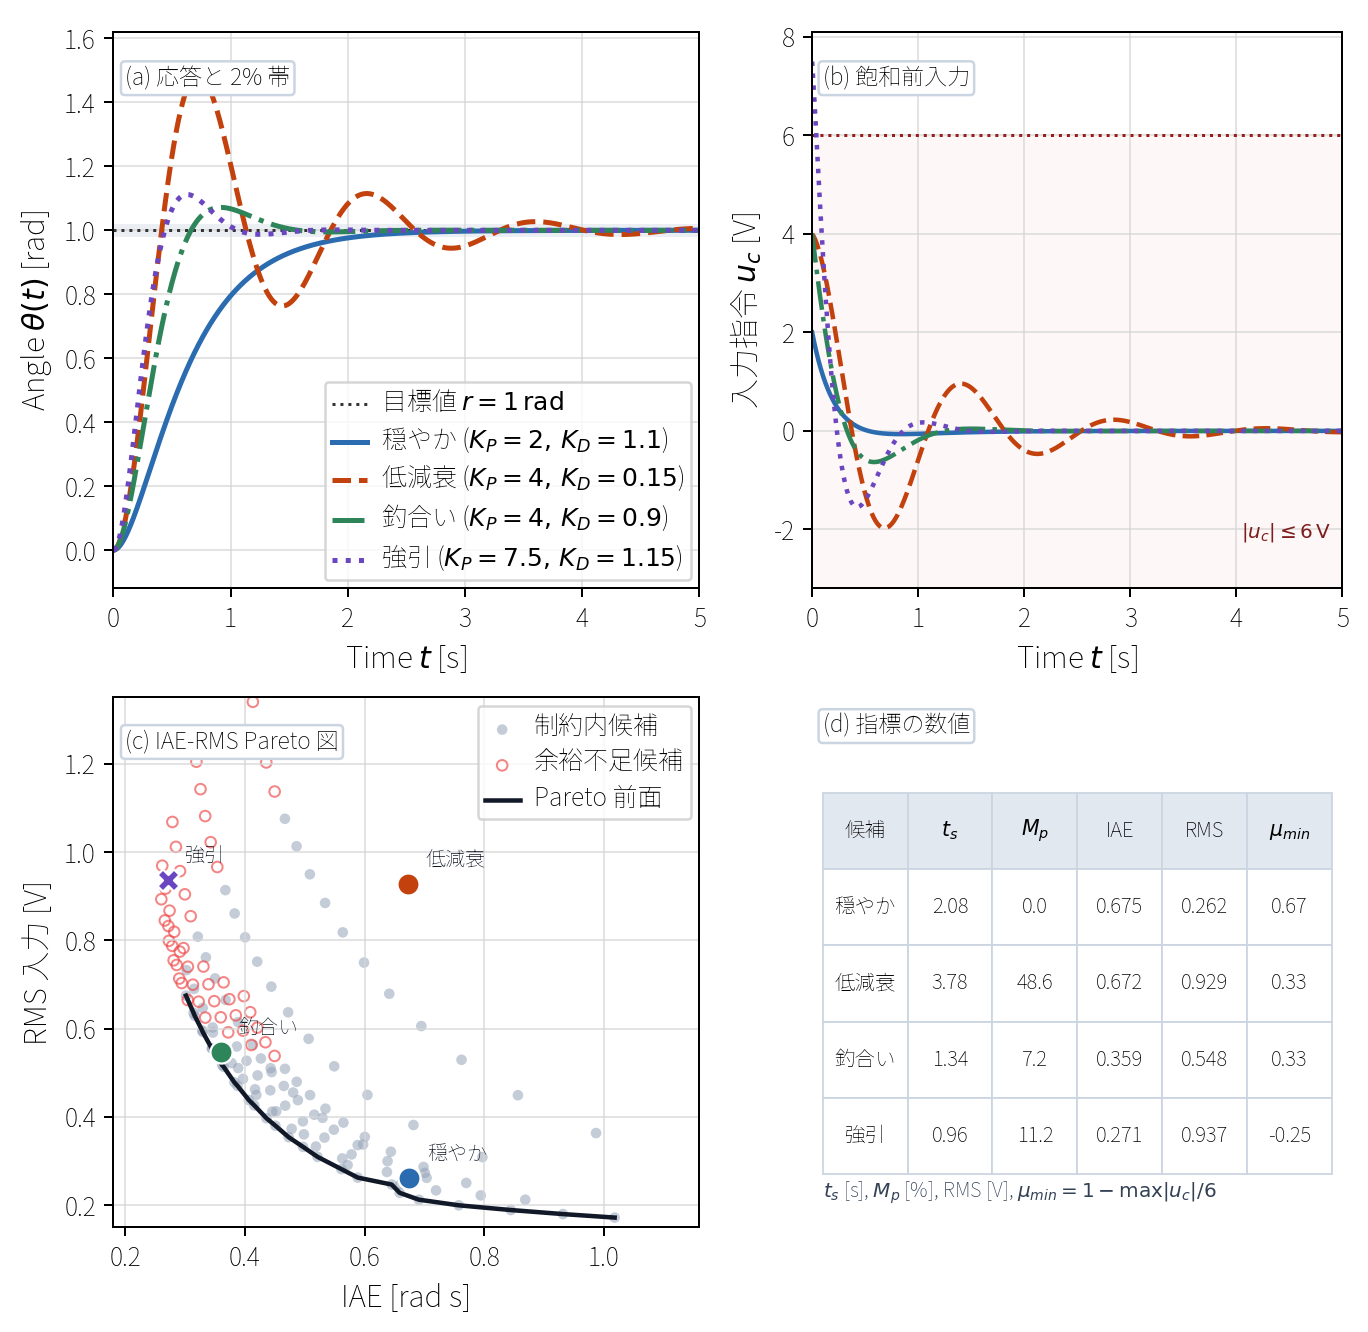
\includegraphics[width=0.98\linewidth,bb=0 0 1368 1332]{figures/performance_pareto_examples.png}
\caption{DC モータ位置サーボに対する性能指標と Pareto 図。対象は $J=0.20\,\mathrm{kg\,m^2}$、$b=0.25\,\mathrm{N\,m\,s/rad}$、$K_t=1.0\,\mathrm{N\,m/V}$、入力制約は $|u|\leq6.0\,\mathrm{V}$、目標値は $r=1.0\,\mathrm{rad}$ である。上段は応答と飽和前入力、下段左は多数の $K_P,K_D$ 候補を IAE と RMS 入力で比べた Pareto 図、下段右は代表候補の指標表である。}
\label{fig:performance-pareto-examples}
\end{figure}

同じ結果を数値表にすると、波形だけでは見落としやすい差がはっきりする。評価時間は $T=5.0\,\mathrm{s}$、整定帯は目標値の $2\%$ とした。$U_{\mathrm{rms}}$、$U_{\mathrm{pk}}$、$\mu_{\min}$ は飽和前入力 $u_c$ から計算している。
\begin{table}[tbp]
\centering
\caption{PD 候補の性能指標}
\label{tab:performance-indices-pareto}
\begingroup
\small
\setlength{\tabcolsep}{3pt}
\begin{tabular}{c|ccrrrrrr}
\hline
候補 & $t_s$ [s] & $M_p$ [\%] & IAE & ISE & ITAE & $U_{\mathrm{rms}}$ [V] & $U_{\mathrm{pk}}$ [V] & $\mu_{\min}$\\
\hline
穏やか & 2.08 & 0.0 & 0.675 & 0.412 & 0.356 & 0.262 & 2.00 & 0.67\\
低減衰 & 3.78 & 48.6 & 0.672 & 0.300 & 0.621 & 0.929 & 4.00 & 0.33\\
釣合い & 1.34 & 7.2 & 0.359 & 0.231 & 0.106 & 0.548 & 4.00 & 0.33\\
強引 & 0.96 & 11.2 & 0.271 & 0.169 & 0.066 & 0.937 & 7.50 & -0.25\\
\hline
\end{tabular}
\endgroup
\end{table}

低減衰の候補は、穏やかな候補と IAE がほぼ同じであるにもかかわらず、オーバーシュートは $48.6\%$、ITAE は $0.621$、RMS 入力は $0.929\,\mathrm{V}$ まで増えている。つまり、初期には速く動くが、後半まで振動が残るため、時間重み付きの偏差と入力要求の両方で不利になる。釣合いの候補は低減衰の候補と同じ $U_{\mathrm{pk}}=4.00\,\mathrm{V}$ で、制約余裕も同じ $0.33$ である。それでも $K_D$ を増やして減衰を足すだけで、$t_s$ は $3.78\,\mathrm{s}$ から $1.34\,\mathrm{s}$ へ短くなり、ITAE は $0.621$ から $0.106$ へ下がる。この比較では、低減衰の候補は釣合いの候補に支配されている。

強引な候補は IAE、ISE、ITAE のすべてが最小で、整定時間も $0.96\,\mathrm{s}$ と最短である。しかし $U_{\mathrm{pk}}=7.50\,\mathrm{V}$ であり、$\mu_{\min}=-0.25$ である。これは、制御器が上限の $1.25$ 倍の電圧を要求したことを意味する。飽和器を通した実入力は $6.0\,\mathrm{V}$ に制限されるので、表の速さは「入力制約を無視してよい」という結論ではない。むしろ、制約余裕を指標に入れないと、物理的に無理な候補を最良に見せてしまうことを示している。

\subsubsection{Pareto 図とスカラー評価への接続}

複数の指標を同時に小さくしたいとき、まず支配される候補を落とす。候補 $a$ と $b$ を IAE と RMS 入力で比べ、$a$ の IAE が $b$ 以下で、かつ $a$ の RMS 入力も $b$ 以下であり、少なくとも一方が厳密に小さいなら、$a$ は $b$ を支配する。このとき $b$ を選ぶ理由は、少なくともこの二つの指標だけからはない。

\wfig{performance-pareto-examples} の下段左は、$K_P$ と $K_D$ を広く変えた候補群を IAE と RMS 入力の平面に置いたものである。左下へ行くほど偏差も入力も小さいが、すべての点が左下へ同時に移れるわけではない。制約内候補の Pareto 前面では、IAE を小さくするほど RMS 入力が増えやすい。穏やかな候補は入力が小さい側、釣合いの候補は偏差と入力の中間、強引な候補は偏差が小さい側にある。ただし強引な候補は制約余裕が負なので、制約を満たす候補としては扱えない。

この図は、スカラー評価が自動的に一つへ決まるものではなく、設計者が何を重く見るかを入れる手段であることを表している。例えば正の正規化定数 $t_0,M_0,A_0,E_0,TA_0,U_0$ を用意し、候補 $i$ に対して
\begin{align}
  J_i(w)
  &=
  w_T\frac{t_{s,i}}{t_0}
  +w_M\frac{M_{p,i}}{M_0}
  +w_A\frac{\mathrm{IAE}_i}{A_0}
  +w_E\frac{\mathrm{ISE}_i}{E_0}
  +w_{TA}\frac{\mathrm{ITAE}_i}{TA_0} \notag\\
  &\quad
  +w_R\frac{U_{\mathrm{rms},i}}{U_0}
  +w_P\frac{U_{\mathrm{pk},i}}{u_{\max}}
  +w_C\max(0,-\mu_{\min,i})
  \label{eq:scalar-cost-from-indices}
\end{align}
と置く。重み $w_T,w_M,w_A,w_E,w_{TA},w_R,w_P,w_C$ はすべて非負である。入力余裕を強く守るなら $w_C$ と $w_P$ を大きくする。後半まで残る偏差を避けたいなら $w_{TA}$ を大きくする。ピークの行き過ぎを嫌う機械なら $w_M$ を大きくする。どの重みでも支配された候補が選ばれにくいことは同じだが、Pareto 前面上のどこを選ぶかは重みで変わる。

この段階で重要なのは、スカラー評価を作っただけでは制御則が突然得られるわけではない、という点である。式 \weq{scalar-cost-from-indices} は、すでに作った候補を後から採点する評価である。次の段階では、候補ゲインを並べる代わりに、いまこの瞬間に入れる入力そのものを評価関数で選ぶ。サンプリング時刻 $k$ の状態を $x_k=[\theta_k\ \omega_k]^\T$ とし、離散化した予測モデルを
\begin{equation}
  x_{k+1}=f_d(x_k,u_k)
\end{equation}
と書く。一段先だけを見る最小の形は
\begin{align}
  J_1(u_k;x_k)
  &=
  q_e(r_{k+1}-\theta_{k+1})^2
  +q_\omega\omega_{k+1}^2
  +r_u\left(\frac{u_k}{u_{\max}}\right)^2
  +r_\Delta\left(\frac{u_k-u_{k-1}}{u_{\max}}\right)^2,\\
  u_k^\ast
  &=
  \arg\min_{|u_k|\leq u_{\max}} J_1(u_k;x_k)
  \label{eq:one-step-horizon-bridge}
\end{align}
である。式 \weq{one-step-horizon-bridge} の構成を、性能指標と Pareto 図から一段の有限ホライズン評価へ移る橋渡しとして \wfig{one-step-horizon-bridge} に示す。図では現在状態 $x_k$ から、制約 $|u_k|\leq u_{\max}$ の中にある複数の候補入力を試し、それぞれで予測される次状態 $x_{k+1}$ と評価成分を並べている。

\begin{figure}[tbp]
\centering
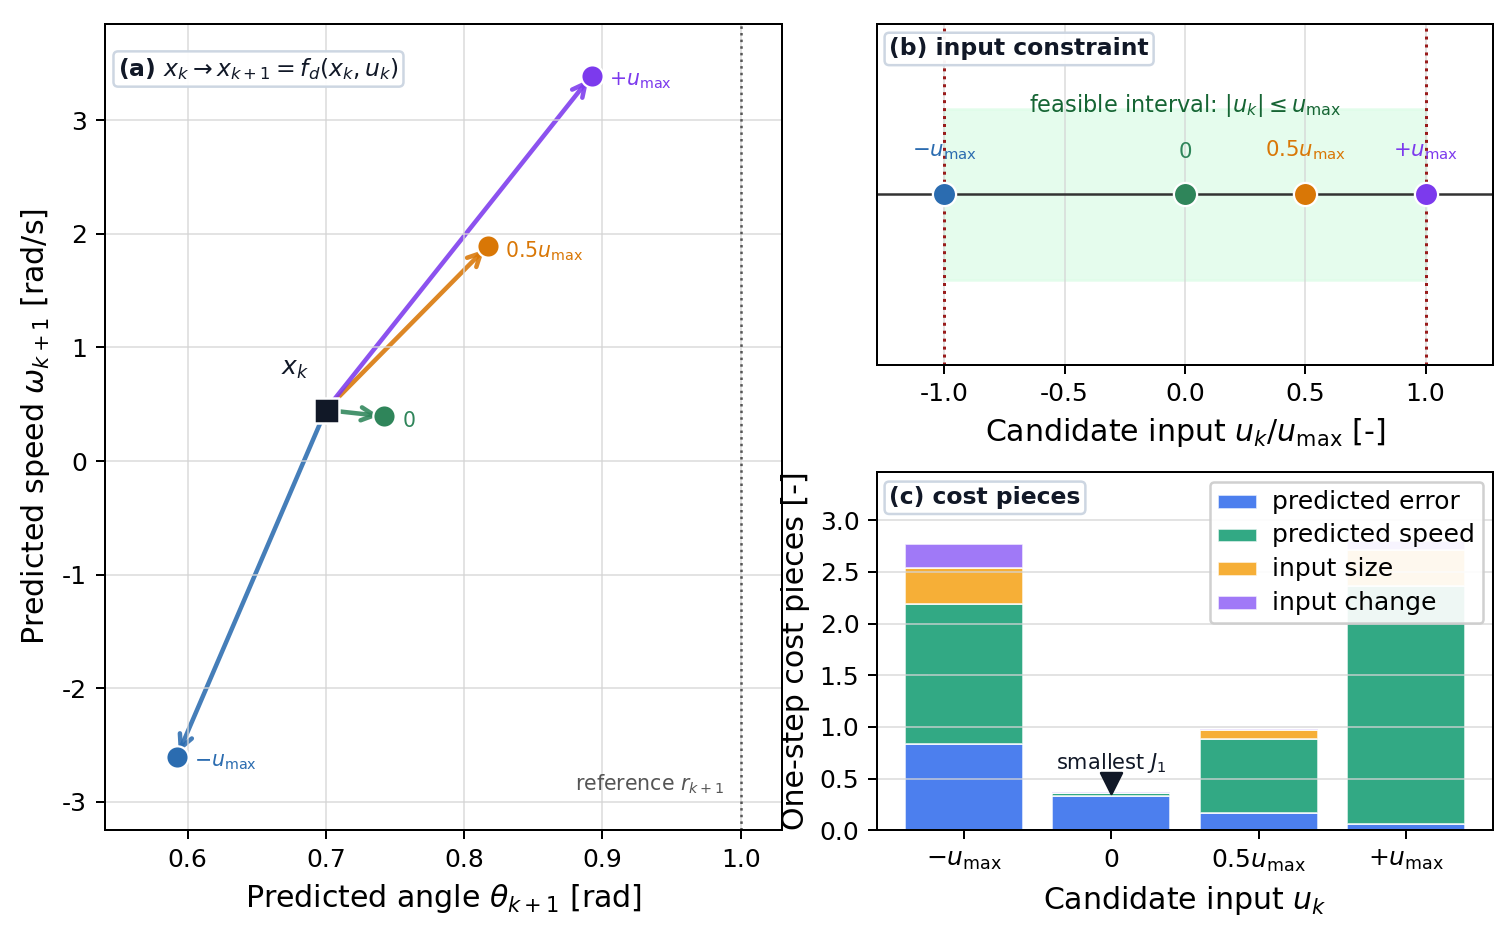
\includegraphics[width=0.98\linewidth,bb=0 0 1512 936]{figures/one_step_horizon_bridge.png}
\caption{性能指標と Pareto 図から作ったスカラー評価を、一段先の入力選択として読むための橋渡し図。現在状態 $x_k$、候補入力 $u_k$、予測された次状態 $x_{k+1}$、入力制約 $|u_k|\leq u_{\max}$、および偏差・速度・入力・入力変化の評価成分を同時に示している。この図は性能指標と Pareto 採点から有限ホライズンの見方へ移る一段の可視化であり、LQR や MPC の導出ではない。}
\label{fig:one-step-horizon-bridge}
\end{figure}

ここでは、未来を一段だけ予測し、次の偏差、次の速度、入力の大きさ、入力変化を同じスカラー評価に入れている。性能指標と Pareto 図で見た「偏差を減らすほど入力が増える」という関係が、この一段先の最適入力選択では評価関数の中へ移る。ただし、この段落の目的は LQR や MPC へ進むことではなく、候補全体を後から採点していた見方を、いま選ぶ入力 $u_k$ の採点へ一段だけ近づけることである。まずこの一段先の形で、重みと制約が入力選択をどう変えるかを読む準備が整う。
